\documentclass{beamer}
\usepackage[utf8]{inputenc}
\usepackage[T1]{fontenc} 
\title{CS 581: Blockchain Science and Technology}
%\date[ISPN '80]{27th International Symposium of Prime Numbers}
\titlegraphic{\includegraphics[width=2cm]{logos/logo.pdf}}
%\author[Euclid]{Euclid of Alexandria \texttt{euclid@alexandria.edu}}
\usepackage[most]{tcolorbox}
\usepackage{multirow}
\usepackage{xcolor}
\usetheme{guwahati}

\lstdefinestyle{mystyle}{
  basicstyle=\ttfamily\scriptsize,
  breaklines=true,
  frame=single,
  numbers=left
}

\lstset{style=mystyle}

\begin{document}


\begin{frame}
  \titlepage
\end{frame}

\frame{
  \frametitle{Course Objectives}

\begin{tcolorbox}

  Bitcoin is the first \textcolor{red}{decentralized  cryptocurrency}. Nodes in the peer-to-peer bitcoin network verify transactions through cryptography and record them in a \textcolor{red}{public distributed ledger}, called a blockchain, \textcolor{red}{ without central oversight}

 \flushright \textit{Wikipedia}

 \end{tcolorbox}
\only<2->{
 Understand each of those ``features'', the tradeoffs involved and generalize when possible.}
}

\frame{
  \frametitle{Lecture Plan}
  
\begin{itemize}
 \item<1-> Currency/Money
 \item<2-> Permissionless Digital Identity
 \item<3-> Hashing
\end{itemize}

}

\frame{
  \frametitle{Currency}
  
\begin{itemize}
 \item<1->  Everyone deposits  their assets at a central godown.
 \item<2->  The godown issues certificates.
 \item<3->  People trade the certificates.
 \item<4->  Anyone can redeem the certificates for the underlying anytime.
 \item<5->  Standardize the certificates.
 \item<6->  Build electronic exchanges for trade.
\end{itemize}
}

\frame{
  \frametitle{Simplified Currency }
\begin{itemize}
 \item Just one type of asset!
 \item The certificate contains just a number.
\end{itemize}
  
}


\frame{
  \frametitle{Ledger for currency(First Attempt)}

  \begin{tcolorbox}[colback=white,colframe=black,width=0.8\textwidth]
    \begin{center}
      

\begin{tabular}{|c|c|c|}
\hline
\multicolumn{3}{|c|}{Universal Cash Positions}\tabularnewline
\hline
\hline
  \multicolumn{3}{|c|}{}\tabularnewline
  \multicolumn{3}{|c|}{}\tabularnewline
\hline
Name & Value & Remark\tabularnewline
\hline
 Aadarshraj& 35 & \tabularnewline
\hline
 Amjad&  87& \tabularnewline
\hline
 Gunjan&  -43& \tabularnewline
\hline
 Harsh& -34  & \tabularnewline
\hline
\end{tabular}
    \end{center}



    
  \end{tcolorbox}

}


\frame{
  \frametitle{Digital Identity via PKC}
\only<1->{
  \begin{tcolorbox}
    We can find $e$, $d$ and $n$ such that

    $$(m)^{ed} \equiv (m) \mod n $$
  \end{tcolorbox}
}



\only<2->{
   \begin{tcolorbox}
    Knowing $e$, and $n$ such that doesn't help in computing $d$.
  \end{tcolorbox}
}
}
\frame{
  \frametitle{RSA Cryptosystem}
  
\begin{itemize}
 \item Choose large primes $p$ and $q$. Let $n=pq$
 \item Choose large $d$ s.t $gcd(d, \phi(n)) = 1$.
 \item Fix $e$ as inverse of  $d$ ( $mod \phi(n)$)
 \end{itemize}

  \begin{tcolorbox}
  $(m)^{ed} = (m)^{k*\phi(n) +1}= (m^{\phi(n)})^{k}\times m = m \mod n$
  \end{tcolorbox}
 
}

\frame{
  \frametitle{Immutability via Hashing}

\begin{figure}[ht]
    \centering
    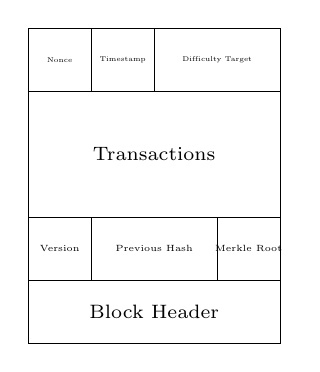
\begin{tikzpicture}[scale=0.8]
        % Block
        \draw (0,0) rectangle (4,1);
        \node at (2,0.5) {\scriptsize Block Header};
        
        % Version
        \draw (0,1) rectangle (1,2);
        \node at (0.5,1.5) {\scalebox{.65}{\tiny Version}};
        
        % Previous Hash
        \draw (1,1) rectangle (3,2);
        \node at (2,1.5){\scalebox{.65}{\tiny Previous Hash}};
        
        % Merkle Root
        \draw (3,1) rectangle (4,2);
        \node at (3.5,1.5) {\scalebox{.65}{\tiny Merkle Root}};
        
        % Transactions
        \draw (0,2) rectangle (4,4);
        \node at (2,3) {\scriptsize Transactions};
        
        % Nonce
        \draw (0,4) rectangle (1,5);
        \node at (0.5,4.5) {\scalebox{.5}{\tiny Nonce}};
        
        % Timestamp
        \draw (1,4) rectangle (2,5);
        \node at (1.5,4.5) {\scalebox{.5}{\tiny Timestamp}};
        
        % Difficulty Target
        \draw (2,4) rectangle (4,5);
        \node at (3,4.5) {\scalebox{.5}{\tiny Difficulty Target}};
    \end{tikzpicture}
    \caption{Bitcoin Block Structure}
    \label{fig:block_structure}
\end{figure}
  
}

\frame{
  \frametitle{}

\begin{figure}[ht]
    \centering
    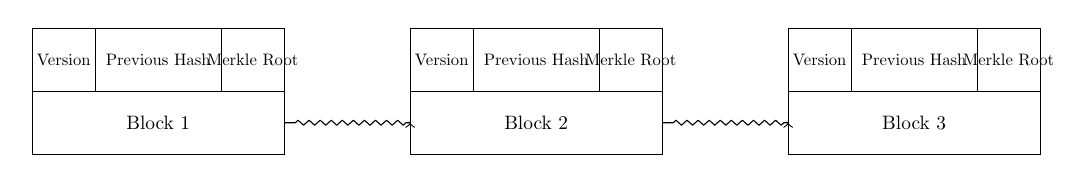
\begin{tikzpicture}[scale=0.8]
        % Block 1
        \draw (0,0) rectangle (4,1);
        \node at (2,0.5) {\scalebox{0.7}{Block 1}};
        
        % Version
        \draw (0,1) rectangle (1,2);
        \node at (0.5,1.5) {\scalebox{0.6}{Version}};
        
        % Previous Hash
        \draw (1,1) rectangle (3,2);
        \node at (2,1.5) {\scalebox{0.6}{Previous Hash}};
        
        % Merkle Root
        \draw (3,1) rectangle (4,2);
        \node at (3.5,1.5) {\scalebox{0.6}{Merkle Root}};
        
        % Zigzag pointer 1
        \draw[->, line join=round, decorate, decoration={zigzag,segment length=4,amplitude=.9,pre=lineto,pre length=4pt}] (4,0.5) -- (6,0.5);
        
        % Block 2
        \draw (6,0) rectangle (10,1);
        \node at (8,0.5) {\scalebox{0.7}{Block 2}};
        
        % Version
        \draw (6,1) rectangle (7,2);
        \node at (6.5,1.5) {\scalebox{0.6}{Version}};
        
        % Previous Hash
        \draw (7,1) rectangle (9,2);
        \node at (8,1.5) {\scalebox{0.6}{Previous Hash}};
        
        % Merkle Root
        \draw (9,1) rectangle (10,2);
        \node at (9.5,1.5) {\scalebox{0.6}{Merkle Root}};
        
        % Zigzag pointer 2
        \draw[->, line join=round, decorate, decoration={zigzag,segment length=4,amplitude=.9,pre=lineto,pre length=4pt}] (10,0.5) -- (12,0.5);
        
        % Block 3
        \draw (12,0) rectangle (16,1);
        \node at (14,0.5) {\scalebox{0.7}{Block 3}};
        
        % Version
        \draw (12,1) rectangle (13,2);
        \node at (12.5,1.5) {\scalebox{0.6}{Version}};
        
        % Previous Hash
        \draw (13,1) rectangle (15,2);
        \node at (14,1.5) {\scalebox{0.6}{Previous Hash}};
        
        % Merkle Root
        \draw (15,1) rectangle (16,2);
        \node at (15.5,1.5) {\scalebox{0.6}{Merkle Root}};
        
    \end{tikzpicture}
    \caption{Bitcoin Blocks with Zigzag Pointers}
    \label{fig:blocks_with_pointers}
\end{figure}
  
}
\end{document}

 